\documentclass[runningheads]{llncs}
\usepackage{amsmath}
\usepackage{amsfonts}
\usepackage{booktabs}
\usepackage[compress]{cite}
\usepackage{color}
\usepackage{graphicx}
\usepackage{hyperref}

\renewcommand\UrlFont{\color{blue}\rmfamily}

\begin{document}

\title{
    Ukraine Conflict Similar Tweets
}
\author{Gabriele Cerizza}
\authorrunning{G. Cerizza}

\institute{Università degli Studi di Milano\\
\email{gabriele.cerizza@studenti.unimi.it}\\
\url{https://github.com/gabrielecerizza/amd_project}}

\maketitle

\section*{Introduction}
\label{sec:introduction}

In this report we detail our findings in the study of an algorithm capable of identifying pairs of similar documents within massive datasets.

In Section~\ref{sec:dataset} we illustrate the dataset and the adopted pre-processing techniques. In Section~\ref{sec:models} we briefly describe the algorithm and its implementation. We also outline the neural network used as comparison. In Section~\ref{sec:experiments} we provide comments on our experiments. Finally, Section~\ref{sec:conclusions} contains our concluding remarks.

\section{Dataset}
\label{sec:dataset}

In this section we provide an overview of the dataset (Section~\ref{subsec:dataset:description}) and of the pre-processing techniques (Section~\ref{subsec:dataset:preprocessing}).

\subsection{Description}
\label{subsec:dataset:description}

The dataset employed in our experiments was the “Ukraine Conflict Twitter Dataset" from Kaggle\footnote{\url{www.kaggle.com/datasets/bwandowando/ukraine-russian-crisis-twitter-dataset-1-2-m-rows}}, released under the CC BY-NC-SA 4.0 license. We assume the reader to be familiar with the terminology associated with Twitter, including expressions such as “tweet", “retweet", “hashtag", and “handle"\footnote{We refer to \url{https://help.twitter.com/en/resources/glossary} for a quick review of the terminology.}.

This dataset boasts over 40 million tweets concerning the conflict between Russia and Ukraine, which broke out on the 24$^{\text{th}}$ of February 2022. Those tweets were collected daily by monitoring hashtags. The dataset was first published on the 27$^{\text{th}}$ of February 2022. In the remainder of this report, we will refer to the version 127 of the dataset, downloaded on the 19$^{\text{th}}$ of June 2022. 

The dataset comprises 109 compressed CSV files. For each sampled tweet, among others, we can find information concerning the author, the text, the hashtags, the language and the date of creation of the messages. We used the \texttt{text} field to extract each document and the \texttt{language} field to select only English documents. 

It is worth noting that the naming format of the files is not consistent. As a consequence, sorting the files lexicographically by file name, the first files contain tweets from April, despite the presence of other files containing tweets from February and March.

\subsection{Filtering and Pre-processing}
\label{subsec:dataset:preprocessing}

The dataset contains a sizeable number of retweets or tweets that differ only for the inclusion of a number or emoji or handle or punctuation symbol or URL. Tweets consisting only of hashtags or very short messages are likewise abundant. Given the nature of Twitter, this is to be expected. However, such documents do not provide a substantial challenge to models aimed at retrieving similar documents, given the amount of identical, overlapping text. For this reason, we set out to remove as much as possible those documents by way of a first filtering phase. The documents were then further pre-processed before being fed to the models.

\subsubsection{Filtering.} Filtering was carried out by performing the following operations: 

\begin{enumerate}
  \item we removed URLs;
  \item we removed handles;
  \item we replaced words with accents with their counterparts without accents;
  \item we replaced special UNICODE characters with their ASCII counterparts, for instance “$\mathbb{R}$" with “R";
  \item we replaced the ampersand with “and";
  \item we converted everything to lowercase;
  \item we removed non-ASCII characters, except for cyrillic characters;
  \item we removed punctuation symbols;
  \item we removed stop words;
  \item we normalized the white space;
  \item we dropped documents shorter than 100 characters.
\end{enumerate}

These steps were performed having two objectives in mind: (i) dropping duplicates, after discarding noisy and irrelevant information; and (ii) reducing the number of different characters that could be found in the tweets. Indeed, a high number of different characters could require the employment of hash functions that adversely affect the execution time of the main algorithm (see Sections~\ref{subsec:experiments:shingles} and~\ref{subsec:experiments:buckets}).
 
\subsubsection{Pre-processing.} Different pre-processing pipelines were applied to the documents given as input to the main algorithm described in Section~\ref{subsec:models:lsh} and to the neural network described in Section~\ref{subsec:models:transformer}.

Concerning the documents given as input to the main algorithm, the filtering steps described above also directly affected the documents and, therefore, may be considered part of the pre-processing pipeline. However, the filtering steps were also used to drop the documents that, after those operations, turned out to be identical. On the contrary, the pre-processing steps described below were not involved in determining whether two documents should be considered identical. These pre-processing steps were:

\begin{enumerate}
  \item using the \texttt{spacy} library\footnote{\url{https://spacy.io/}}, we replaced each token with the corresponding lemma, to increase the match between words like “invasion" and “invaded";
  \item we removed punctuation symbols that were introduced by the lemmatization;
  \item we normalized the white space again.
\end{enumerate}

The documents given as input to the neural network were not affected by the filtering steps, which, in this case, were used solely to drop duplicates. As a consequence, the only pre-processing steps were the following:

\begin{enumerate}
  \item we removed URLs;
  \item we replaced words with accents with their counterparts without accents;
  \item we replaced the ampersand with “and";
  \item we replaced special UNICODE characters with their ASCII counterparts, for instance “$\mathbb{R}$" with “R";
  \item we removed non-ASCII characters, except for cyrillic characters;
  \item we normalized the white space.
\end{enumerate}

We decided to perform a light pre-processing for the neural network in order to leverage its ability to exploit the context of each word, which would have been hampered by removing punctuation and stop words or by lemmatizing the tokens.

Finally, note that, while numbers might be considered noise in some contexts, here we decided to keep them. Indeed, in our context, numbers could be found in dates and military equipment (e.g., the Russian T-72 tank or the M982 Excalibur 155 mm shell) and could help in discriminating the documents.

\section{Models}
\label{sec:models}

In this section we briefly describe the algorithm used to find similar documents (Section~\ref{subsec:models:lsh}) and the neural network used as a baseline to compare performances (Section~~\ref{subsec:models:transformer}). We also propose an example to motivate the comparison between the two models (Section~\ref{subsec:models:motivation}).

\subsection{Locality-Sensitive Hashing Algorithm}
\label{subsec:models:lsh}

In order to find the pairs of similar documents, we employed the locality-sensitive hashing (LSH) algorithm described in~\cite{leskovec_2020}, which can scale up to massive datasets. We assume the reader to be familiar with the algorithm and we provide here only a brief summary. The algorithm converts each document to a set of k-grams (shingles), builds a characteristic matrix and then a signature matrix by using hash functions, applies a LSH technique to find candidate similar pairs and, finally, checks the candidate pairs against the signature matrix to discard false positive pairs. Optionally, one could check the candidate pairs also against the characteristic matrix, if available.

\subsubsection{Hash functions.} Concerning the implementation details, we first discuss the various hash functions exploited by the algorithm. 

To avoid keeping the shingles in main memory, the algorithm hashes each shingle to a bucket, which is associated to an integer. This integer takes less space in memory than the shingle. The total number of buckets associated to the hash function has a significant impact on the execution time (see Section~\ref{subsec:experiments:buckets}). We generated different hash functions by truncating the output of the SHA-256 hash function at varying lengths of bits. In this way, we could experiment with different numbers of buckets.  

The algorithm requires also hash functions that could map a row index to another row index. These hash functions are used to efficiently perform permutations of the rows of the characteristic matrix. Since the number of these hash functions is a hyper-parameter set by the user, we needed a way to generate an arbitrary number of different hash functions. To this end, we followed the approach described in~\cite{liu_2015}, generating hash functions of the form
\[
  h(x) = (ax + b)~\text{mod}~c~,  
\]
where $x$ is a row index, $a$ and $b$ are random numbers smaller than the maximum row index and $c$ is a prime number higher than the maximum row index.

Inside the LSH technique, to check whether two columns of a given band of the signature matrix were equal, we hashed the string composed by the sequence of integers inside each column using the default \texttt{hash} function provided by Python. This allowed us to compress a potentially huge array of numbers into a single number, thus saving main memory space. 

\subsubsection{Characteristic matrix.} In order to build the signature matrix, the algorithm requires a characteristic matrix, where each column represents a document and each entry indicates whether or not a given shingle is contained in a given document. We store the characteristic matrix as a dictionary that maps each document index to its set of shingles. In this way, we do not waste memory to store the null entries.

\subsubsection{LSH.} Concerning the LSH technique, in order to find the number of bands for the signature matrix and the correlated number of rows in each band, we used \texttt{scipy} and solved the system of equations
\begin{equation*}
  \begin{cases}
    t = (\frac{1}{b})^\frac{1}{r}\\
    b \cdot r = n
  \end{cases}\,,
\end{equation*}
where $t$ is a threshold on the required similarity between two documents, $b$ is the number of bands, $r$ is the number of rows in each band and $n$ is the total number of rows of the signature matrix.

\subsubsection{Scalability bottlenecks.} The implementation of the algorithm features two possible scalability bottlenecks. The first one concerns the characteristic matrix. Using 3-grams, 4-grams, 5-grams and 6-grams, each document contained on average 120-130 shingles. If we represented each shingle with a 32-bit integer, processing 10 million documents would require roughly 5 gigabytes of main memory ($\frac{1\text{e}7 \cdot 130 \cdot 32}{8\text{e}9} = 5.2$). Keeping the whole dataset (40 million documents) in main memory might prove challenging or even impossible. A solution could be to store the representations of the documents as sets of shingles in mass memory and read them one at a time when building the signature matrix. However, that would slow down an already time consuming operation, since to build the signature matrix we have to cycle through all the documents for each row of the characteristic matrix.

The second bottleneck concerns the number of similar pairs. The lower the value for the threshold, the higher the number of similar pairs identified by the algorithm. When processing millions of documents, even a moderate threshold might saturate the main memory. A solution could be to store the candidate pairs identified by the LSH technique on mass memory. This would have to happen within each band of the signature matrix and, therefore, we would not be able to have unique pairs: the same pair might be identified and stored on mass memory in more than one band. This would result in redundant processing.

It is also worth noting that the time complexity to build the signature matrix is $\mathcal{O}(R D H)$, where $R$ is the number of rows of the characteristic matrix, $D$ is the number of documents and $H$ is the number of hash functions that perform permutations. Building the signature matrix is the most time consuming operation within the procedure.

\subsection{Neural Network (Transformer)}
\label{subsec:models:transformer}

The dataset did not provide a ground truth against which we could compare our results. Therefore, we decided to use a state-of-the-art model in the field of natural language processing (NLP) to serve as a baseline in determining how similar two documents were. To this end, we opted to use MPNet~\cite{song_2020}, which is a neural network based on the revolutionary BERT Transformer~\cite{vaswani_2017, devlin-etal-2019-bert}.

A Transformer used to obtain word embeddings is similar to word2vec~\cite{mikolov-etal-2013-word2vec}, with one important difference. The difference is that word2vec produces static embeddings, which means that a given word will be mapped to the same vector regardless of its context. On the contrary, the Transformer produces contextualized embeddings, so that we will obtain a different vector for each different context (sentence) in which a given word appears. To give an example, the Transformer would generate different embeddings for the word “mouse" used with the meaning of animal and with the meaning of computer device, whereas word2vec would generate the same embedding.

We used the Transformer to obtain an embedding for each document. First, we extracted a word embedding for each word in a given document by using the last hidden layer of the model, which captures semantic features~\cite{laicher-etal-2021-explaining}. Afterwards, we computed the mean of the word embeddings of the document.

\subsection{Motivation}
\label{subsec:models:motivation}

We motivate our decision to compare the LSH algorithm with a Transformer by showing an example. Consider the following three documents.
\begin{enumerate}
  \item “I went to the bank to withdraw money and compensate the plaintiff for their losses".
  \item “The Russians are withdrawing from the banks of the Dnipro River after suffering heavy losses".
  \item “After the judgement, I had to use my debit card and pay the suer for the damages".
\end{enumerate}
We can see that the first and the third document are semantically related, despite the fact that they do not share many words. On the contrary, the first and the second document are not semantically related, but share words like “bank", “withdraw" and “losses".

We apply a light pre-processing on the documents, consisting in removing punctuation, applying lowercase, performing lemmatization and normalizing the white space. Then, we extract 3-grams and we compute the Jaccard similarity between each pair of documents. Recall that the LSH algorithm produces an estimation of the Jaccard similarity. After that, we compute the cosine similarity between the sentence embeddings extracted from the Transformer, without any pre-processing.

The results are shown in Table~\ref{tab:models:comparison}. As expected, the Jaccard similarity identifies the first and second document as the most similar, whereas the Transformer correctly identifies the first and the third document as the most similar. This suggests that the LSH algorithm may not be able to adequately capture the semantic similarity between documents. Thus, we could use the Transformer to check whether the pairs identified as similar by the LSH algorithm are indeed similar.

\begin{table}
  \caption{Similarity between each pair out of the three documents described in Section~\ref{subsec:models:motivation}, computed by Jaccard similarity on 3-grams and by the Transformer.}
  \label{tab:models:comparison}
  \centering
  \begin{tabular}{lrrr}
      \toprule
      & \multicolumn{3}{c}{Similarity} \\
      \cmidrule{2-4}
      Method & Pair (1,2) & Pair (1,3) & Pair (2,3) \\
      \midrule
      Jaccard Similarity & 0.185 & 0.000 & 0.023\\
      Transformer & 0.192 & 0.648 & 0.131 \\
      \bottomrule
  \end{tabular}
\end{table}

\section{Experiments}
\label{sec:experiments}

In this section, after reviewing some of the metrics used for evaluation (Section~\ref{subsec:experiments:metrics}), we discuss our experiments on the LSH algorithm. These experiments concerned the growth of the number of different shingles and characters as we increased the number of documents (Section~\ref{subsec:experiments:shingles}); the effect of the number of buckets on the hash functions used to map shingles to integers (Section~\ref{subsec:experiments:buckets}); the effect of the threshold on the similarity between pairs (Section~\ref{subsec:experiments:threshold}); the effect of the number of hash functions used to permute the rows of the characteristic matrix (Section~\ref{subsec:experiments:hashes}); a final comparison between the LSH algorithm and the Transformer on 100,000 tweets (Section~\ref{subsec:experiments:100k}).

All the experiments were carried out using the files covering the tweets from the 1$^{\text{st}}$ of April 2022 to the 7$^{\text{th}}$ of April 2022. We selected only the tweets in the English language. We refer to Section~\ref{subsec:dataset:preprocessing} for the filtering and pre-processing techniques adopted. The analyzed files contained around 2 million documents. After the filtering, only 221,615 documents remained. This confirms that the dataset is filled with almost identical or very short tweets. 

The experiments were run on a machine with 16 GB of
RAM and a CPU Intel(R) Core(TM) i7-9700K 3.60GHz with 8 cores.

\subsection{Metrics}
\label{subsec:experiments:metrics}

We define the following metrics: precision, recall, F1-score and mean absolute error (MAE). Within a massive dataset, the number of pairs of dissimilar documents would be preponderant. Therefore, accuracy would likely be very high regardless of the capabilities of the algorithm.
For this reason, we did not consider accuracy. 

In this context, TP is the number of true positive pairs, FP is the number of false positive pairs, and FN is the number of false negative pairs. Those quantities were obtained by computing the actual Jaccard similarity between the documents, which is made possible by directly using the characteristic matrix. Afterwards, we checked if the Jaccard similarity was higher than the threshold.
If the algorithm identified a pair as similar, but the Jaccard similarity did not exceed the threshold, we considered the pair as false positive. If the algorithm identified a pair as similar and the Jaccard similarity exceeded the threshold, we considered the pair as true positive. If the algorithm identified a pair as not similar, but the Jaccard similarity exceeded the threshold, we considered the pair as false negative.

Precision is defined as 
\[
  \text{Precision} = \frac{\text{TP}}{\text{TP} + \text{FP}}\,.
\]

Recall is defined as
\[
  \text{Recall} = \frac{\text{TP}}{\text{TP} + \text{FN}}\,.
\]

F1-score is defined as
\[
  \text{F1-score} = \frac{\text{TP}}{\text{TP} + \frac{1}{2}(\text{FP} + \text{FN})}\,.
\]

MAE is defined as
\[
  \text{MAE} = \frac{1}{N}\sum_{i=1}^N \lvert y_i - x_i \rvert \,,
\]
where $x$ and $y$ are respectively the similarity estimated by the algorithm and the Jaccard similarity computed on the characteristic matrix. Recall that the output of the algorithm is a set of pairs of documents identified as similar. Thus, the algorithm does not provide a similarity value for all the pairs, but only for a subset. This being the case, $N$ is not the total number of pairs, but the number of pairs identified as similar by the algorithm. 

\subsection{Shingles and Characters Growth}
\label{subsec:experiments:shingles}

\begin{figure}
  \center
  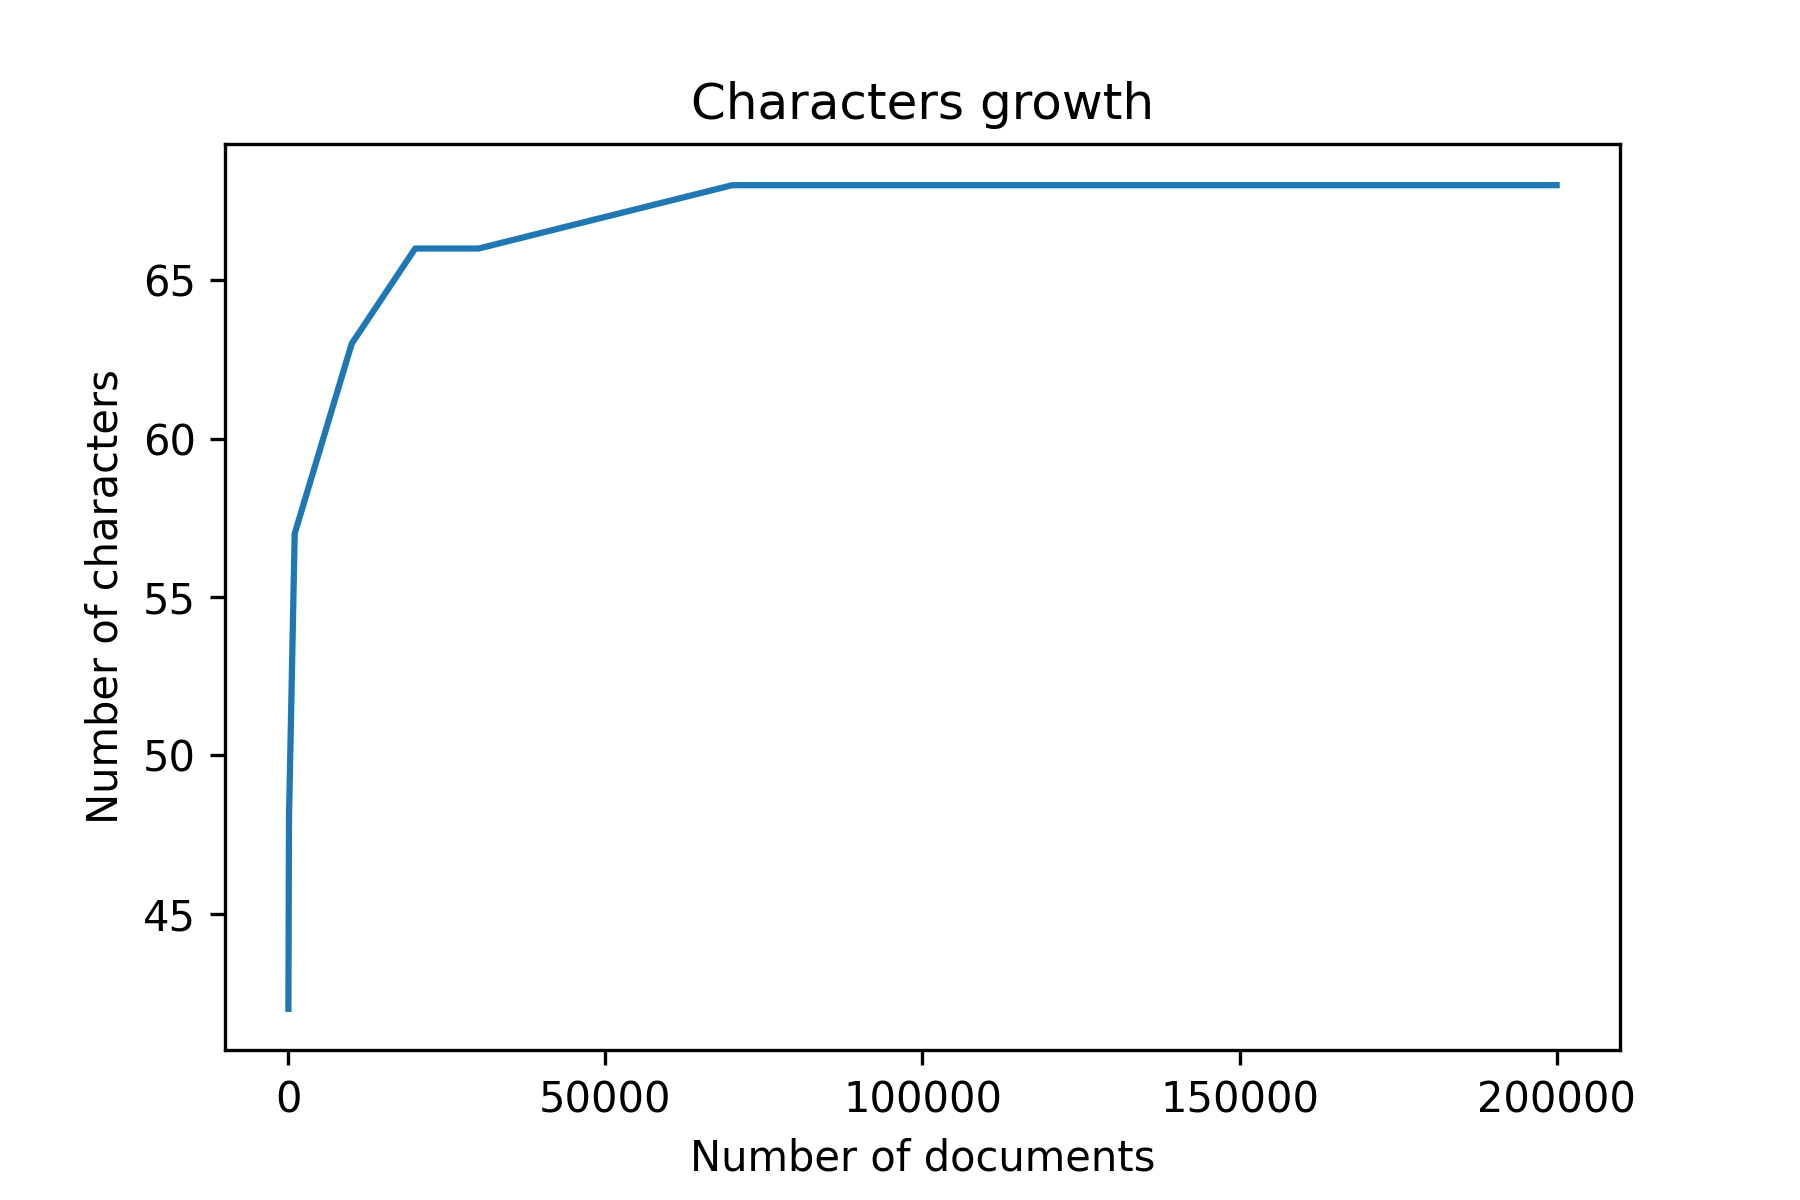
\includegraphics[width=1\textwidth]{../img/char_growth.png}
  \caption{Growth in the number of different characters as the number of documents increased.} 
  \label{fig:experiments:char_growth}
\end{figure}

\begin{figure}
  \center
  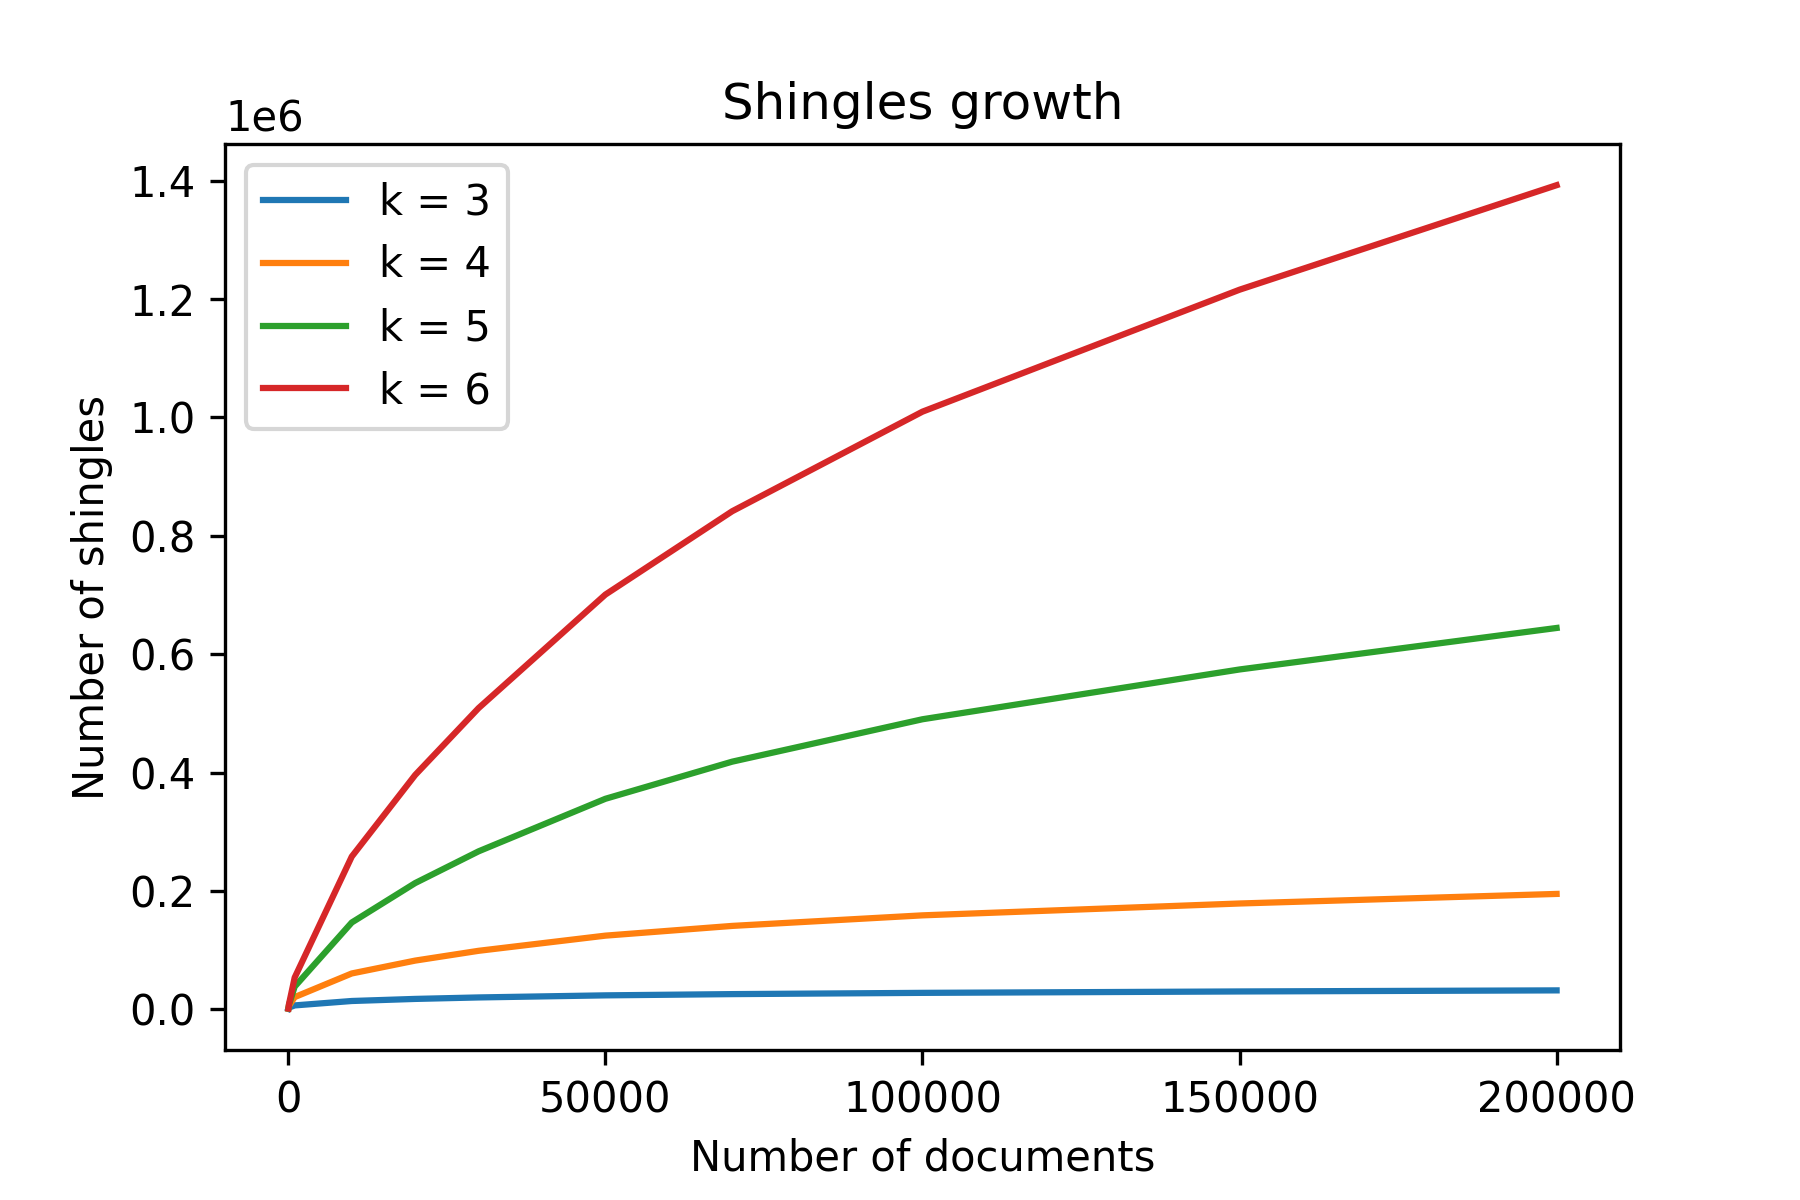
\includegraphics[width=1\textwidth]{../img/shingles_growth.png}
  \caption{Growth in the number of different shingles as the number of documents increased. The growth is shown for shingles obtained with different k-grams.} 
  \label{fig:experiments:shingles_growth}
\end{figure}

In this first experiment we wanted to gauge how the number of different shingles (or k-grams) and characters varied as the number of documents increased.

In Figure~\ref{fig:experiments:char_growth} we can see how the number of different characters grew as the number of documents increased. In particular, we can see how, from 100,000 documents onwards, the number of characters was stable at around 65 characters (68, to be precise). This could be useful to get a hint on the appropriate number of buckets of the hash function that maps k-grams to integers with respect to the chosen k-grams. For instance, given that $68^3 = 314,432$, we can infer that, if we used 3-grams, we would need a hash function with approximately 300,000 buckets.

Working with characters we can get an estimate on the number of buckets that we would need. However, it is unlikely that all the possible shingles will appear in practice. To this end, we also explored how the actual number of different shingles grew as the number of documents increased. This is shown in Figure~\ref{fig:experiments:shingles_growth}. 

It is not surprising to see that, with k-grams having a higher value of k, the number of different shingles grew more steeply. We can also see, however, that this growth was approximately logarithmic in shape and stabilized quickly for low values of k. Indeed, for k equal to 3 and 4, most of the different shingles had already been found at 50,000 documents. To be precise, at 50,000 documents we had 21,580 different shingles with 3-grams and 111,643 different shingles with 4-grams. Accordingly, for 3-grams, a hash function with buckets of at least 15 bits would be enough ($2^{15} = 32,768$ buckets). For 4-grams, we would need at least 17 bits to have a fair chance at avoiding collisions ($2^{17} = 131,072$ buckets). We will see, however, that collisions do not affect the performance as badly as one might expect (see Sections~\ref{subsec:experiments:buckets} and~\ref{subsec:experiments:100k}).

% The following experiments will concern mainly 3-grams, 4-grams and 5-grams. Recall that a suitable value of k should give a low probability of finding a given shingle inside a document. On this account, we remark that even with 3-grams the probability of finding a given shingle inside a document would be low. An upper bound on the total number of different shingles in a document is the number of characters in that document. For tweets, that would be 280 characters. Considering 68 possible different characters, the total number of different shingles would be $68^3 = 314,432$. So, at most, the probability of finding a given shingle would be $\frac{280}{68^3} \approx 0.0008$.

\subsection{Number of Buckets}
\label{subsec:experiments:buckets}

In this experiment we wanted to see how increasing the number of bits, and thus the number of buckets, of the hash function that maps k-grams to integers affected various metrics. The experiment was carried out with a fixed threshold of 0.1, 100 hash functions for the permutations of the rows and a corpus of 100 documents.  

The results are shown in Tables~\ref{tab:experiments:buckets_k3}, \ref{tab:experiments:buckets_k4} and \ref{tab:experiments:buckets_k5} for 3-grams, 4-grams and 5-grams, respectively. We can formulate the following observations.

\begin{itemize}
  \item Using a higher number of bits did not always yield a better result. For instance, we can see that with 3-grams 12 bits yielded the best F1-score.  Although the corpus was limited to 100 documents, this might still suggest that collisions do not affect significantly the performance.
  \item Across all the different numbers of bits, 3-grams obtained high values of F1-score most consistently. 
  \item The higher the value of k in k-grams, the lower the number of pairs estimated as similar. This is to be expected and, indeed, with 1-grams we would find that almost all documents are similar.
  \item Increasing the number of bits raised the execution time. With 22 bits, processing 100 documents took roughly 25 minutes. Coupled with a huge number of documents, this might make working with a high number of buckets prohibitive from the perspective of execution time.  
\end{itemize}

\begin{table}
  \caption{Effects of the increase in the number of bits for the hash function that maps k-grams to integers when k is equal to 3. We highlighted in bold the best results.}
  \label{tab:experiments:buckets_k3}
  \centering
  \begin{tabular}{lcccccc}
    \toprule
    {} &  Pairs No. &  Recall &  Precision &  F1-Score &    MAE & Time Delta \\
    Hash Bits &            &         &            &           &        &            \\
    \midrule
    12        &       2166 &   0.775 &      \textbf{0.678} &     \textbf{0.723} &  0.025 &    0:00:04 \\
    14        &       2008 &   0.823 &      0.569 &     0.673 &  0.029 &    0:00:08 \\
    16        &       1761 &   0.815 &      0.579 &     0.677 &  \textbf{0.023} &    0:00:24 \\
    18        &        995 &   0.525 &      0.634 &     0.574 &  \textbf{0.023} &    0:01:29 \\
    19        &       1564 &   0.730 &      0.559 &     0.633 &  0.030 &    0:03:02 \\
    20        &       2108 &   \textbf{0.866} &      0.492 &     0.628 &  0.033 &    0:05:53 \\
    22        &       1125 &   0.594 &      0.632 &     0.612 &  \textbf{0.023} &    0:23:25 \\
    \bottomrule
    \end{tabular}
\end{table}

\begin{table}
  \caption{Effects of the increase in the number of bits for the hash function that maps k-grams to integers when k is equal to 4. We highlighted in bold the best results.}
  \label{tab:experiments:buckets_k4}
  \centering
  \begin{tabular}{lcccccc}
    \toprule
    {} &  Pairs No. &  Recall &  Precision &  F1-Score &    MAE & Time Delta \\
    Hash Bits &            &         &            &           &        &            \\
    \midrule
    12        &        404 &   0.656 &      0.317 &     0.427 &  0.030 &    0:00:03 \\
    14        &        187 &   0.598 &      0.326 &     0.422 &  0.030 &    0:00:07 \\
    16        &        237 &   0.820 &      0.308 &     0.448 &  0.031 &    0:00:24 \\
    18        &        245 &   0.782 &      0.278 &     0.410 &  0.032 &    0:01:32 \\
    19        &        353 &   \textbf{0.828} &      0.204 &     0.327 &  0.039 &    0:03:06 \\
    20        &        348 &   0.690 &      0.172 &     0.276 &  0.039 &    0:06:37 \\
    22        &        191 &   0.747 &      \textbf{0.340} &     \textbf{0.468} &  \textbf{0.029} &    0:23:55 \\
    \bottomrule
    \end{tabular}
\end{table}

\begin{table}
  \caption{Effects of the increase in the number of bits for the hash function that maps k-grams to integers when k is equal to 5. We highlighted in bold the best results.}
  \label{tab:experiments:buckets_k5}
  \centering
  \begin{tabular}{lcccccc}
    \toprule
    {} &  Pairs No. &  Recall &  Precision &  F1-Score &    MAE & Time Delta \\
    Hash Bits &            &         &            &           &        &            \\
    \midrule
    12        &        206 &   \textbf{0.750} &      0.277 &     0.404 &  0.035 &    0:00:03 \\
    14        &         66 &   0.581 &      0.379 &     0.459 &  0.023 &    0:00:07 \\
    16        &         79 &   0.703 &      0.329 &     0.448 &  0.034 &    0:00:29 \\
    18        &         64 &   0.714 &      0.391 &     0.505 &  0.034 &    0:01:31 \\
    19        &         23 &   0.457 &      \textbf{0.696} &     0.552 &  \textbf{0.022} &    0:03:05 \\
    20        &         31 &   0.600 &      0.677 &     \textbf{0.636} &  0.026 &    0:05:51 \\
    22        &         52 &   0.571 &      0.385 &     0.460 &  0.029 &    0:23:42 \\
    \bottomrule
    \end{tabular}
\end{table}

\subsection{Threshold}
\label{subsec:experiments:threshold}

In this experiment we wanted to see how the value of the threshold affected the predictions. The experiment was carried out with a 16 bits hash function for the mapping between shingles and integers, 100 hash functions for the permutations of the rows and a corpus of 100 documents.

The results are shown in Tables~\ref{tab:experiments:threshold_k3}, \ref{tab:experiments:threshold_k4} and \ref{tab:experiments:threshold_k5} for 3-grams, 4-grams and 5-grams, respectively. We can formulate the following observations.

\begin{itemize}
  \item Above a certain threshold, the algorithm reached a perfect F1-score for all the k-grams. In general, the algorithm behaved better when the threshold was either very low or very high. This is reasonable, since those are the easiest cases: when almost all pairs are similar or when only almost identical documents are similar.
  \item Increasing the threshold decreased the number of estimated similar pairs, as expected. However, this effect was stronger for k-grams with higher values of k.
  \item MAE got worse as the threshold increased. This could be attributed to the lower number of estimated similar pairs. 
\end{itemize}

\begin{table}
  \caption{Effects of the increase in the threshold value when working with 3-grams. We highlighted in bold the best results.}
  \label{tab:experiments:threshold_k3}
  \centering
  \begin{tabular}{lccccc}
    \toprule
    {} &  Pairs No. &  Recall &  Precision &  F1-Score &    MAE \\
    Threshold &            &         &            &           &        \\
    \midrule
    0.05      &       4067 &   0.924 &      0.941 &     0.932 &  \textbf{0.018} \\
    0.10      &       1761 &   0.815 &      0.579 &     0.677 &  0.023 \\
    0.15      &        242 &   0.582 &      0.236 &     0.335 &  0.037 \\
    0.20      &         23 &   0.750 &      0.261 &     0.387 &  0.043 \\
    0.25      &          4 &   \textbf{1.000} &      0.750 &     0.857 &  0.032 \\
    0.30      &          1 &   \textbf{1.000} &      \textbf{1.000} &     \textbf{1.000} &  0.070 \\
    0.50      &          1 &   \textbf{1.000} &      \textbf{1.000} &     \textbf{1.000} &  0.070 \\
    \bottomrule
    \end{tabular}
\end{table}

\begin{table}
  \caption{Effects of the increase in the threshold value when working with 4-grams. We highlighted in bold the best results.}
  \label{tab:experiments:threshold_k4}
  \centering
  \begin{tabular}{lrrrrr}
    \toprule
    {} &  Pairs No. &  Recall &  Precision &  F1-Score &    MAE \\
    Threshold &            &         &            &           &        \\
    \midrule
    0.05      &       1819 &   0.791 &      0.650 &     0.714 &  \textbf{0.016} \\
    0.10      &        237 &   0.820 &      0.308 &     0.448 &  0.031 \\
    0.15      &         25 &   0.875 &      0.280 &     0.424 &  0.050 \\
    0.20      &          8 &   \textbf{1.000} &      0.375 &     0.545 &  0.058 \\
    0.25      &          2 &   \textbf{1.000} &      0.500 &     0.667 &  0.071 \\
    0.30      &          1 &   \textbf{1.000} &      \textbf{1.000} &     \textbf{1.000} &  0.108 \\
    0.50      &          1 &   \textbf{1.000} &      \textbf{1.000} &     \textbf{1.000} &  0.108 \\
    \bottomrule
    \end{tabular}
\end{table}

\begin{table}
  \caption{Effects of the increase in the threshold value when working with 5-grams. We highlighted in bold the best results.}
  \label{tab:experiments:threshold_k5}
  \centering
  \begin{tabular}{lccccc}
    \toprule
    {} &  Pairs No. &  Recall &  Precision &  F1-Score &    MAE \\
    Threshold &            &         &            &           &        \\
    \midrule
    0.05      &       1035 &   0.808 &      0.414 &     0.548 &  \textbf{0.019} \\
    0.10      &         79 &   0.703 &      0.329 &     0.448 &  0.034 \\
    0.15      &         10 &   \textbf{1.000} &      0.300 &     0.462 &  0.052 \\
    0.20      &          3 &   \textbf{1.000} &      0.333 &     0.500 &  0.060 \\
    0.25      &          1 &   \textbf{1.000} &      \textbf{1.000} &     \textbf{1.000} &  0.111 \\
    0.30      &          1 &   \textbf{1.000} &      \textbf{1.000} &     \textbf{1.000} &  0.111 \\
    0.50      &          1 &   \textbf{1.000} &      \textbf{1.000} &     \textbf{1.000} &  0.111 \\
    \bottomrule
    \end{tabular}
\end{table}

\subsection{Number of Hash Functions}
\label{subsec:experiments:hashes}

In this experiment we wanted to verify how the number of hash functions used to perform permutations affected the algorithm. The experiment was carried out with a 16 bits hash function for the mapping between shingles and integers, a threshold value of 0.1 and a corpus of 100 documents.

The results are shown in Tables~\ref{tab:experiments:hashes_k3}, \ref{tab:experiments:hashes_k4} and \ref{tab:experiments:hashes_k5} for 3-grams, 4-grams and 5-grams, respectively. We can formulate the following observations.

\begin{itemize}
  \item Increasing the number of hash functions decreased the number of pairs estimated as similar and increased the precision. The effect is similar to what we observed in the threshold experiment, but with a significant difference. Here we can see how recall got progressively worse as we increased the number of hash functions. The takeaway is not to increase drastically the number of hash functions and not to rely on the sole precision to evaluate the algorithm. This will be important for our final experiment, because in that context we will be unable to measure recall and F1-score due to the huge number of documents (see Section~\ref{subsec:experiments:100k}). 
  \item 200 hash functions seemed to strike a good compromise between precision and recall across all the different k-grams.
  \item The increase in execution time, when working with a higher number of hash functions, was negligible.
\end{itemize}


\begin{table}
  \caption{Effects of the increase in the number of hash functions used to perform permutations when working with 3-grams. We highlighted in bold the best results.}
  \label{tab:experiments:hashes_k3}
  \centering
  \begin{tabular}{lcccccc}
    \toprule
    {} &  Pairs No. &  Recall &  Precision &  F1-Score &    MAE & Time Delta \\
    Hash No. &            &         &            &           &        &            \\
    \midrule
    20       &       1793 &   0.577 &      0.403 &     0.474 &  0.045 &    0:00:19 \\
    100      &       1761 &   \textbf{0.815} &      0.579 &     \textbf{0.677} &  0.023 &    0:00:24 \\
    200      &       1468 &   0.725 &      0.619 &     0.668 &  0.023 &    0:00:31 \\
    300      &         74 &   0.046 &      0.770 &     0.086 &  \textbf{0.019} &    0:00:36 \\
    500      &          1 &   0.001 &      \textbf{1.000} &     0.002 &  0.032 &    0:00:45 \\
    \bottomrule
    \end{tabular}
\end{table}

\begin{table}
  \caption{Effects of the increase in the number of hash functions used to perform permutations when working with 4-grams. We highlighted in bold the best results.}
  \label{tab:experiments:hashes_k4}
  \centering
  \begin{tabular}{lcccccc}
    \toprule
    {} &  Pairs No. &  Recall &  Precision &  F1-Score &    MAE & Time Delta \\
    Hash No. &            &         &            &           &        &            \\
    \midrule
    20       &        951 &   0.798 &      0.075 &     0.137 &  0.057 &    0:00:21 \\
    100      &        237 &   \textbf{0.820} &      0.308 &     0.448 &  0.031 &    0:00:25 \\
    200      &        137 &   0.775 &      0.504 &     \textbf{0.611} &  0.020 &    0:00:34 \\
    300      &         17 &   0.169 &      \textbf{0.882} &     0.283 &  \textbf{0.014} &    0:00:40 \\
    500      &          0 &   0.000 &      0.000 &     0.000 &  0.000 &    0:00:45 \\
    \bottomrule
    \end{tabular}
\end{table}

\begin{table}
  \caption{Effects of the increase in the number of hash functions used to perform permutations when working with 5-grams. We highlighted in bold the best results.}
  \label{tab:experiments:hashes_k5}
  \centering
  \begin{tabular}{lcccccc}
    \toprule
    {} &  Pairs No. &  Recall &  Precision &  F1-Score &    MAE & Time Delta \\
    Hash No. &            &         &            &           &        &            \\
    \midrule
    20       &        772 &   \textbf{0.703} &      0.034 &     0.064 &  0.068 &    0:00:19 \\
    100      &         79 &   \textbf{0.703} &      0.329 &     0.448 &  0.034 &    0:00:25 \\
    200      &         36 &   0.514 &      0.528 &     \textbf{0.521} &  \textbf{0.030} &    0:00:29 \\
    300      &          3 &   0.081 &      \textbf{1.000} &     0.150 &  0.043 &    0:00:33 \\
    500      &          0 &   0.000 &      0.000 &     0.000 &  0.000 &    0:00:43 \\
    \bottomrule
    \end{tabular}
\end{table}

\subsection{Similarity Between 100,000 Tweets}
\label{subsec:experiments:100k}

For this last experiment, we compared the results of the algorithm with different configurations of hyper-parameters against the Transformer. We used the Transformer to compute the similarity only between the pairs selected by the LSH algorithm. After that, we compared the rank-order correlation between the similarities computed by the two models using Kendall's Tau and Spearman's Rho. Both Kendall's Tau and Spearman's Rho range from -1 to +1, where -1 means strong disagreement, 0 means no correlation and +1 means strong agreement. We also considered precision and MAE, as defined in Section~\ref{subsec:experiments:metrics}. We forwent recall and F1-score, which would require to compute the similarity between all the possible pairs of documents, due to the high number of documents.

The results are shown in Table~\ref{tab:experiments:d100k}. We can formulate the following observations.

\begin{itemize}
  \item The strongest correlations were obtained by using 3-grams.
  \item Surprisingly, even with 12-bits hash functions the algorithm achieved a good performance. This supports our hypothesis that collisions have a limited impact on the performance. Additionally, with 12-bits hash functions the algorithm is able to churn out results at a fast rate (around one hour for 100,000 documents).   
  \item In general, the similarity values computed by the algorithm showed only a moderate positive correlation with the similarity values computed by the Transformer. Therefore, we can conclude that the pairs of documents estimated as similar by the algorithm may be lacking a semantic association.
  \item Increasing both the threshold and the number of hash functions on 3-grams deteriorated the performance of the algorithm.
  \item With 5-grams, the algorithm returned almost half of the pairs that we got using 3-grams and the same threshold. We already discussed in Section~\ref{subsec:experiments:buckets} how higher values of k in k-grams naturally produce a lower number of similar pairs. However, as we mentioned in Section~\ref{subsec:experiments:hashes}, this experiment might also suggest that, despite the high precision, the algorithm working on 5-grams produced a high number of false negatives. 
\end{itemize}

In Table~\ref{tab:experiments:examples} we provide examples of similar documents identified by the algorithm having the best Kendall's Tau correlation in Table~\ref{tab:experiments:d100k}. Note how, despite the heavy filtering, these documents are almost identical. Note also how the practice of filling tweets with hashtags may result in an artificial similarity. Unfortunately, removing hashtags from the documents would render moot any comparison between tweets. 

\begin{table}
  \caption{Performance of the algorithm on a corpus of 100,000 documents. Kendall's Tau and Spearman's Rho correlations used the Transformer described in Section~\ref{subsec:models:transformer} to compare the similarity values. We highlighted in bold the best results.}
  \label{tab:experiments:d100k}
  \centering
  \begin{tabular}{llllccccc}
    \toprule
      &     &     &    &  Pairs No. &  Prec. &    MAE &  Kendall &  Spearman \\
    K & T & Hash No. & Hash Bits &            &        &        &          &           \\
    \midrule
    3 & 0.6 & 200 & 16 &     174941 &  0.956 &  0.023 &    0.229 &     \textbf{0.323} \\
      3 & 0.8 & 300 & 16 &      30917 &  0.903 &  \textbf{0.015} &    0.076 &     0.109 \\
      3 & 0.6 & 200 & 12 &     163221 &  0.967 &  0.020 &    \textbf{0.230} &     0.319 \\
      3 &   0.6  & 100 & 12 &     182562 &  0.940 &  0.029 &    0.219 &     0.304 \\
    4 & 0.6 & 200 & 18 &     112186 &  0.961 &  0.022 &    0.136 &     0.192 \\
    4  &   0.6  &  200   & 12 &     108446 &  0.976 &  0.022 &    0.148 &     0.205 \\
    5 & 0.6 & 200 & 16 &      94191 &  0.900 &  0.027 &    0.143 &     0.202 \\
    5  &  0.6   &  200   & 12 &      82153 &  \textbf{0.977} &  0.022 &    0.115 &     0.161 \\
    \bottomrule
    \end{tabular}
\end{table}

\begin{table}
  \caption{Examples of similar documents identified by the algorithm having the best Kendall's Tau correlation in Table~\ref{tab:experiments:d100k}.}
  \label{tab:experiments:examples}
  \centering
  \begin{tabular}{p{0.35\textwidth}@{\hspace{0.5cm}}p{0.35\textwidth}@{\hspace{0.5cm}}r}
    \toprule
     Doc. 1 & Doc. 2 & Similarity \\
    \midrule
    \#Russia’s President Vladimir \#Putin says he has signed a decree saying foreign buyers must pay in rubles for Russian gas from April 1, and contracts would be halted if these payments are not made. \url{https://t.co/IUBuHMgw4n} & Russian President Vladimir \#Putin said on Thursday that he has signed a decree saying foreign buyers must pay in roubles for Russian gas from the first of \#April and contracts would be halted if these payments were not made. \url{https://t.co/BApCaIiaOo} & 0.810 \\
    \hline
    An oil depot is on fire in \#Belgorod, \#Russia. “The emergency services went to the place of fire, measures are being taken to eliminate it", said Gladkov, the governor of the region in his Telegram channel. \url{https://t.co/ey7rC5ChSz} & Horrible Video- An oil depot is on \#fire in \#Belgorod, \#Russia. “The \#emergency services went to the place of fire, measures are being taken to eliminate it", said \#Gladkov, the governor of the region in his Telegram channel.\#RussianWarCrimes \#UkraineRussianWar \url{https://t.co/WmqRo7LkaT} & 0.805 \\
    \hline
    If Putin is to be tried for war crimes, of course he can’t remain in power \url{https://t.co/CGmEEQlRu7} \#HolocaustMemorialDay \#MLK \#GrenfellTower \#BidenHarris \#BlackLivesMatter  \#OprahMeghanHarry \#ReparationsNow \#Zelensky \#Ukraine \#Kyiv \#karkhiv \#Odesa \#Lviv \#Mariupol \#Lutsk \#Dnipro & Putin's white privilege Prosecuting war crimes demands outrage, will and action \url{https://t.co/3vbAFtqjY0} \#HolocaustMemorialDay \#MLK \#GrenfellTower \#BidenHarris \#BlackLivesMatter  \#OprahMeghanHarry \#ReparationsNow \#Zelensky \#Ukraine \#Kyiv \#karkhiv \#Kherson \#Odesa \#Lviv \#Mariupol & 0.635\\
    \hline
    @sputnikint @russiatoday @moscowtimes @moscowgov @emb\_rus @russia Other 134,000 young \#Russia conscript as soldiers to be sent by the old corrupt \#Putin to die in \#Ukraine, not for their homeland but only for  personal glory and enrichment of Putin and his gang. Is it worth it ? \url{https://t.co/O4VH6KINOK} & @russiatoday @russiaun @russianembassy @sputnikint @russiabeyond\_it @russia @moscowtimes @russia Do the new 134,000 young men from \#Russia conscripted by \#Putin know that they go to die in \#Ukraine not for their homeland but only for glory and enrichment of Putin and his gang? \url{https://t.co/Ii2vebZOGf} & 0.635\\
    \bottomrule
  \end{tabular}
\end{table}


\section{Conclusions}
\label{sec:conclusions}

This work investigated the performance of the LSH algorithm described in Section~\ref{subsec:models:lsh} across different configurations of hyper-parameters. The algorithm proved to be effective at processing massive amounts of data and at properly estimating the Jaccard similarity between documents. This is the field in which the algorithm excels. A neural network would not be able to compute the pairwise similarity between each pair of documents in a massive dataset. That would require an unreasonable amount of time.

The main pitfall of the algorithm is that Jaccard similarity on k-grams, as shown in Section~\ref{subsec:models:motivation}, might not capture semantic similarity between documents. Given the fact that the algorithm is built on top of a Boolean characteristic matrix, this issue may prove difficult to address. The reason is that we cannot exploit state-of-the-art word embeddings, unless we find a way to suitably encode them as sets.

Another critical aspect of the algorithm was the execution time, at least with hash functions having a high number of buckets, as mentioned in Section~\ref{subsec:experiments:buckets}. Indeed, building the signature matrix is a very expensive operation when using those hash functions. In~\cite{leskovec_2020} there are suggestions on how to address this issue, at the cost of a coarser estimation of the Jaccard similarity.

To further improve the execution time, we could also use a non-cryptographic hash function, instead of SHA-256, to generate hash functions with a variable number of buckets.

\section*{Statement}
\textit{I/We declare that this material,
which I/We now submit for assessment, is entirely my/our own work and has not been
taken from the work of others, save and to the extent that such work has been cited and
acknowledged within the text of my/our work. I/We understand that plagiarism, collusion,
and copying are grave and serious offences in the university and accept the penalties that
would be imposed should I engage in plagiarism, collusion or copying. This assignment,
or any part of it, has not been previously submitted by me/us or any other person for
assessment on this or any other course of study.}


\bibliographystyle{splncs04}
\bibliography{bibtex_entries}

\end{document}